\begin{tikzpicture}

\tikzstyle{process} = [rectangle, minimum width=3.5cm, minimum height=1cm, text centered, 
text width=3.5cm, draw=black, fill=yellow!40]

\node (tab1) {%
\begin{tabular}{|l|l|l|}
   \hline
    $X_i$ & $n_i$ & $f_i$ \\ \hline
    6 & 13 & $f_i = n_1/N= 0.43$ \\
    8 & 12 & $f_i = n_2/N= 0.40$ \\
    12 & 5 & $f_i = n_3/N= 0.17$ \\ \hline
    Total & 30 & 1.00\\ \hline
\end{tabular}
};

\node [process] (n1) at (5.5,0) {\textbf{Frecuencia relativa}\vspace{3mm} $\dfrac{frecuencia~absoluta}{No.~total~de~datos}$};

\draw [thick, dashed, -latex](n1) -- (tab1);
\end{tikzpicture}